\documentclass[11pt,a4paper]{article}

\usepackage[spanish,es-nodecimaldot]{babel}
\usepackage[T1]{fontenc}
\usepackage[utf8]{inputenc}
\usepackage{lmodern}
\usepackage{geometry}
\usepackage{graphicx}
\usepackage{float}
\usepackage{hyperref}
\usepackage{enumitem}

\geometry{margin=2.5cm}
\hypersetup{colorlinks=true,linkcolor=black,urlcolor=blue}
\graphicspath{{img/}}

\title{Ataque a una base de datos MySQL}
\author{Javier Siñuka}
\date{23 de septiembre de 2026}

\begin{document}
\maketitle

\section{Objetivo}
Analizar el archivo \texttt{SQL\_Lab.pcap} para reconstruir un ataque de
inyección SQL contra Damn Vulnerable Web Application (DVWA), identificar la
información expuesta y proponer medidas de prevención.

\section{Material y metodología}
Se abrió el PCAP proporcionado con la actividad en Wireshark en el entorno
Linux local. No se utilizó la máquina virtual CyberOps: el análisis se realizó
sobre el mismo archivo suministrado, sin generar tráfico contra el servidor.
Las figuras son capturas reales de Wireshark ejecutado en una pantalla virtual.
Se siguieron los flujos HTTP y se contrastaron los resultados con su extracción
mediante TShark, conservada en la carpeta \texttt{evidencias/}.
Wireshark descomprime las respuestas HTTP con \texttt{Content-Encoding: gzip}
al seguir el flujo HTTP, lo que permite leer su HTML.

\section{Procedimiento y respuestas}
\subsection{Paso 1: direcciones IP y duración}
Las dos direcciones involucradas son \textbf{10.0.2.4}, origen de las solicitudes
del atacante, y \textbf{10.0.2.15}, servidor web que responde por el puerto
TCP 80. La captura contiene 30 paquetes y abarca \textbf{441,807206 segundos}
(7 minutos y 21,807206 segundos). La referencia de la consigna a ocho minutos
es aproximada. El tráfico observado es HTTP entre el cliente y la aplicación;
no es una captura directa de la conexión interna de MySQL.

\begin{figure}[H]
\centering
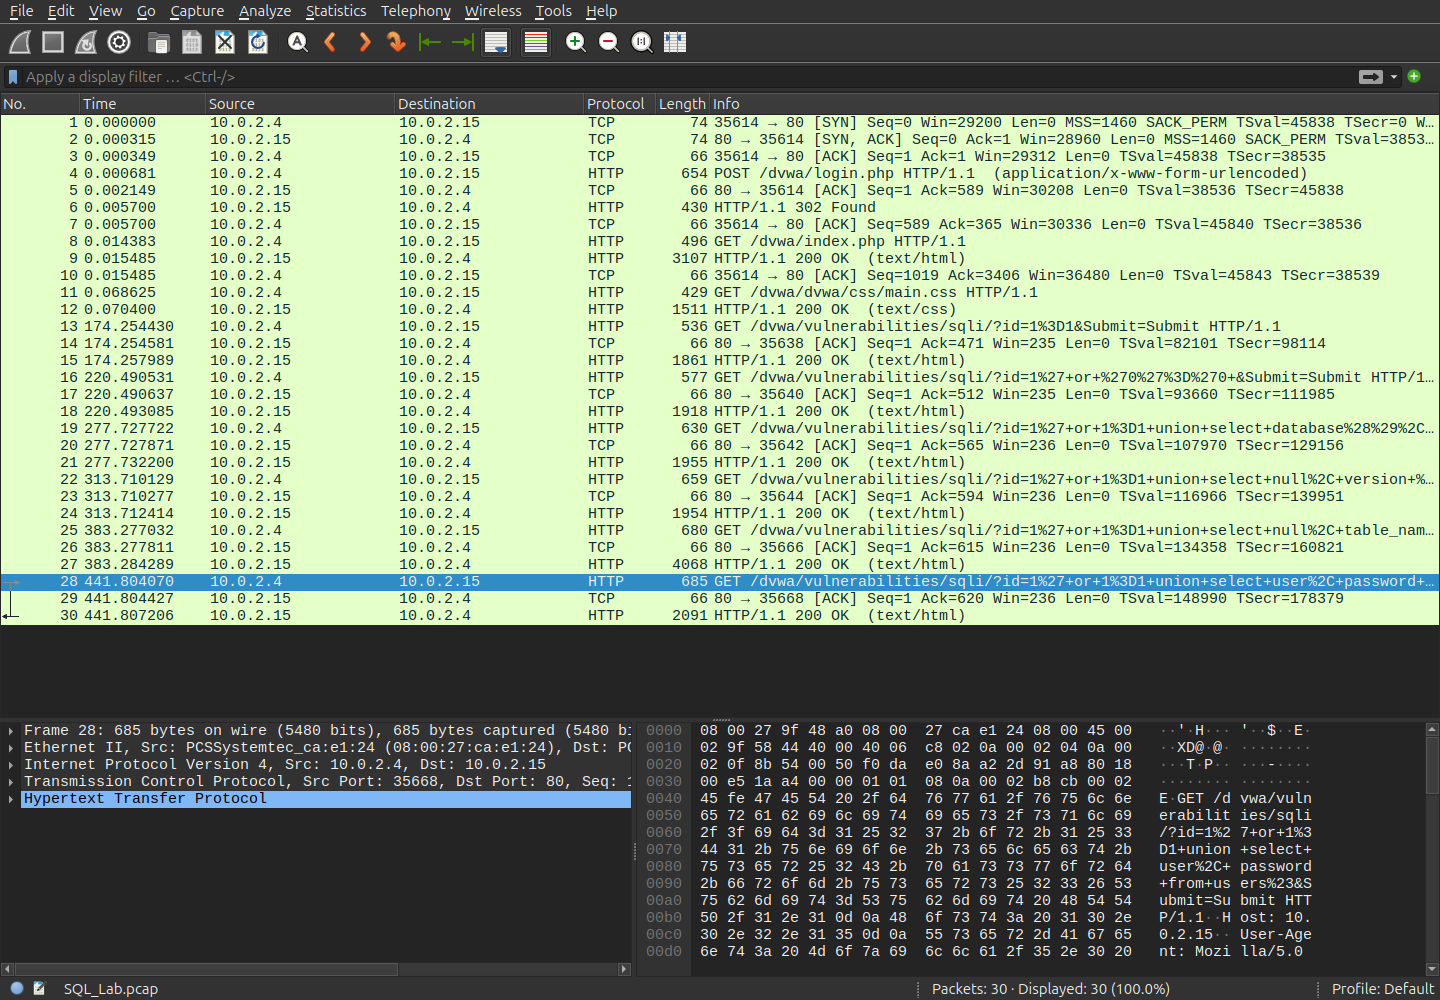
\includegraphics[width=\textwidth]{01_trafico.png}
\caption{PCAP original abierto en Wireshark: direcciones, solicitudes HTTP y tiempos relativos.}
\end{figure}

\subsection{Paso 2: prueba inicial}
El paquete 13 envía el parámetro \texttt{id=1\%3D1}, que decodificado es
\texttt{1=1}. La respuesta del paquete 15 muestra \texttt{First name: admin}
y \texttt{Surname: admin}.

Aunque la consigna presenta esta respuesta como confirmación de una condición
siempre verdadera, la devolución de un registro por sí sola no demuestra cómo
el servidor interpretó esa entrada. La evidencia más clara aparece en el
paquete 16: la entrada \verb|1' or '0'='0 | devuelve los cinco registros de
usuarios en el paquete 18. Posteriormente, las consultas con \texttt{UNION}
confirman la extracción de información adicional. El formulario vulnerable es
una búsqueda por User ID; no debe confundirse con el inicio de sesión.

\begin{figure}[H]
\centering
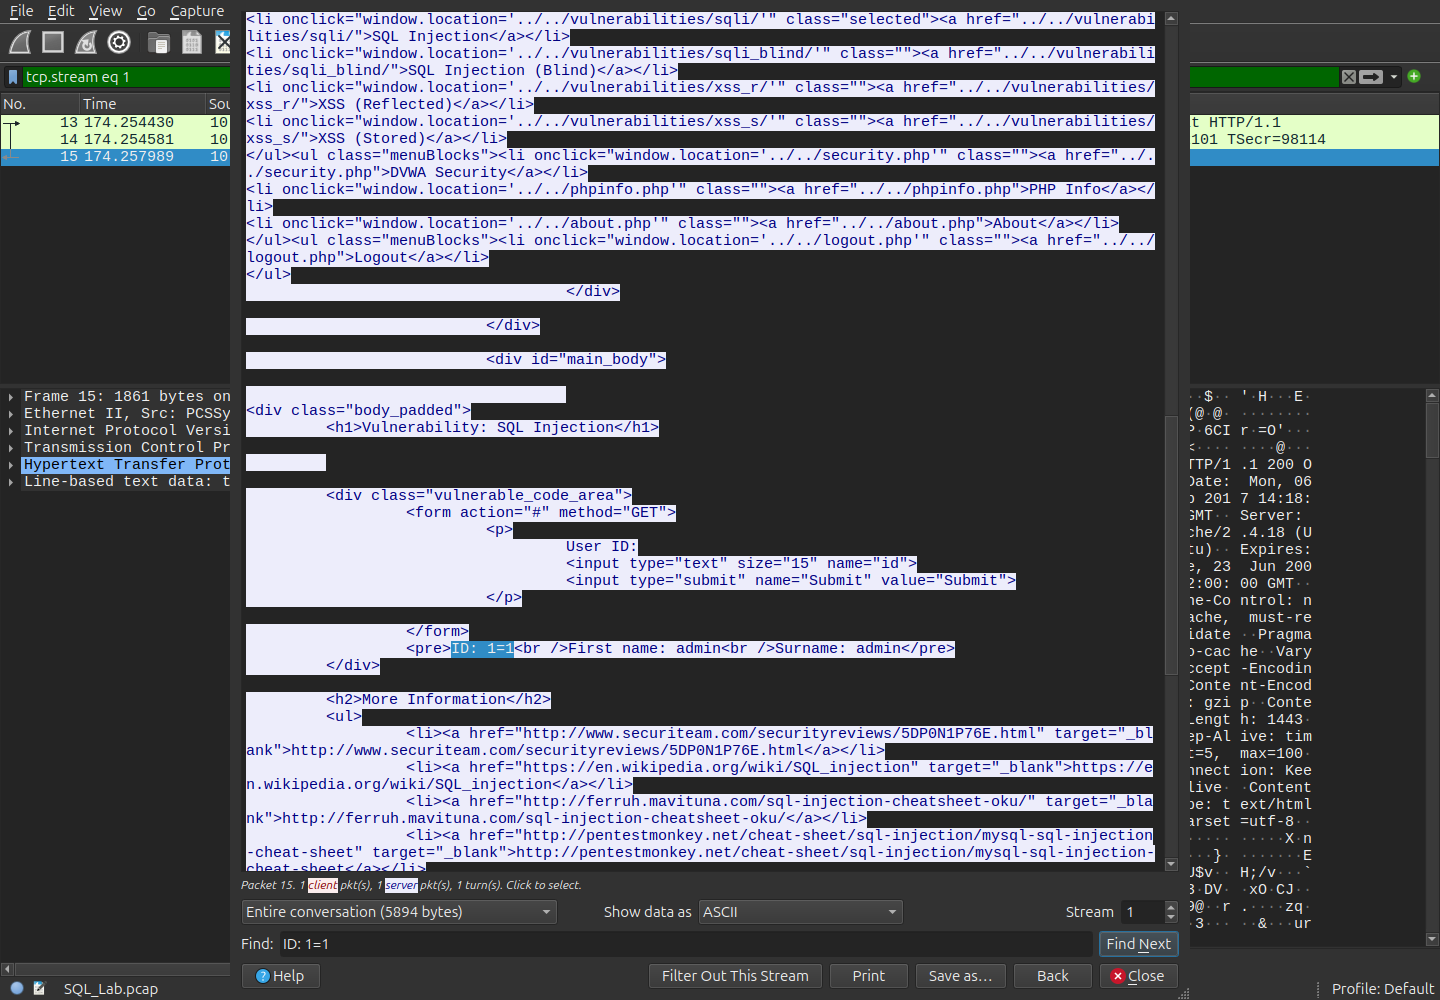
\includegraphics[width=\textwidth]{02_prueba.png}
\caption{Flujo HTTP del paquete 13: entrada 1=1 y registro admin devuelto por el servidor.}
\end{figure}

\subsection{Paso 3: nombre de la base y usuario de conexión}
En el paquete 19 se observa la consulta:
\begin{verbatim}
1' or 1=1 union select database(), user()#
\end{verbatim}
La respuesta del paquete 21 contiene \textbf{dvwa} como base de datos y
\textbf{root@localhost} como usuario de conexión. Este último valor difiere de
\texttt{dvwa@localhost}, indicado en la consigna: se informa el valor comprobado
en el PCAP. El usuario de conexión a MySQL no es necesariamente el usuario
registrado en la aplicación web. El carácter \texttt{\#} comenta el resto de
la sentencia SQL que pudiera agregar la aplicación.

\begin{figure}[H]
\centering
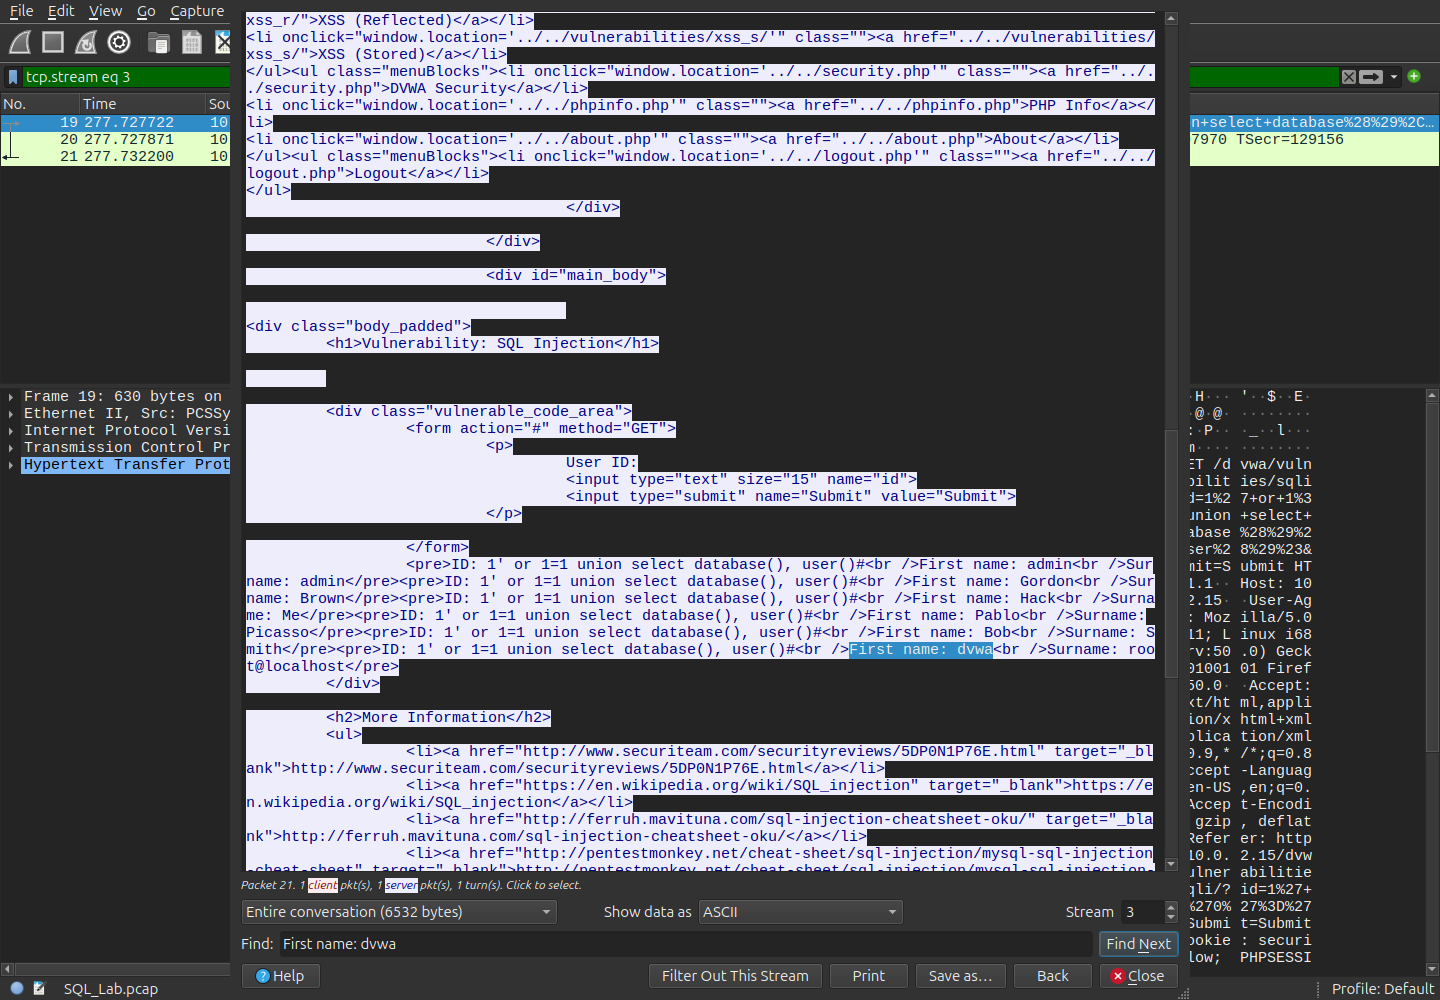
\includegraphics[width=\textwidth]{03_base_usuario.png}
\caption{Respuesta real con la base dvwa y el usuario root@localhost.}
\end{figure}

\subsection{Paso 4: versión del sistema gestor}
El paquete 22 contiene:
\begin{verbatim}
1' or 1=1 union select null, version ()#
\end{verbatim}
La versión devuelta en el paquete 24 es \textbf{5.7.12-0ubuntu1.1}.
\texttt{NULL} ocupa la primera columna y la versión aparece en la segunda,
rotulada \texttt{Surname} por la plantilla HTML.

\begin{figure}[H]
\centering
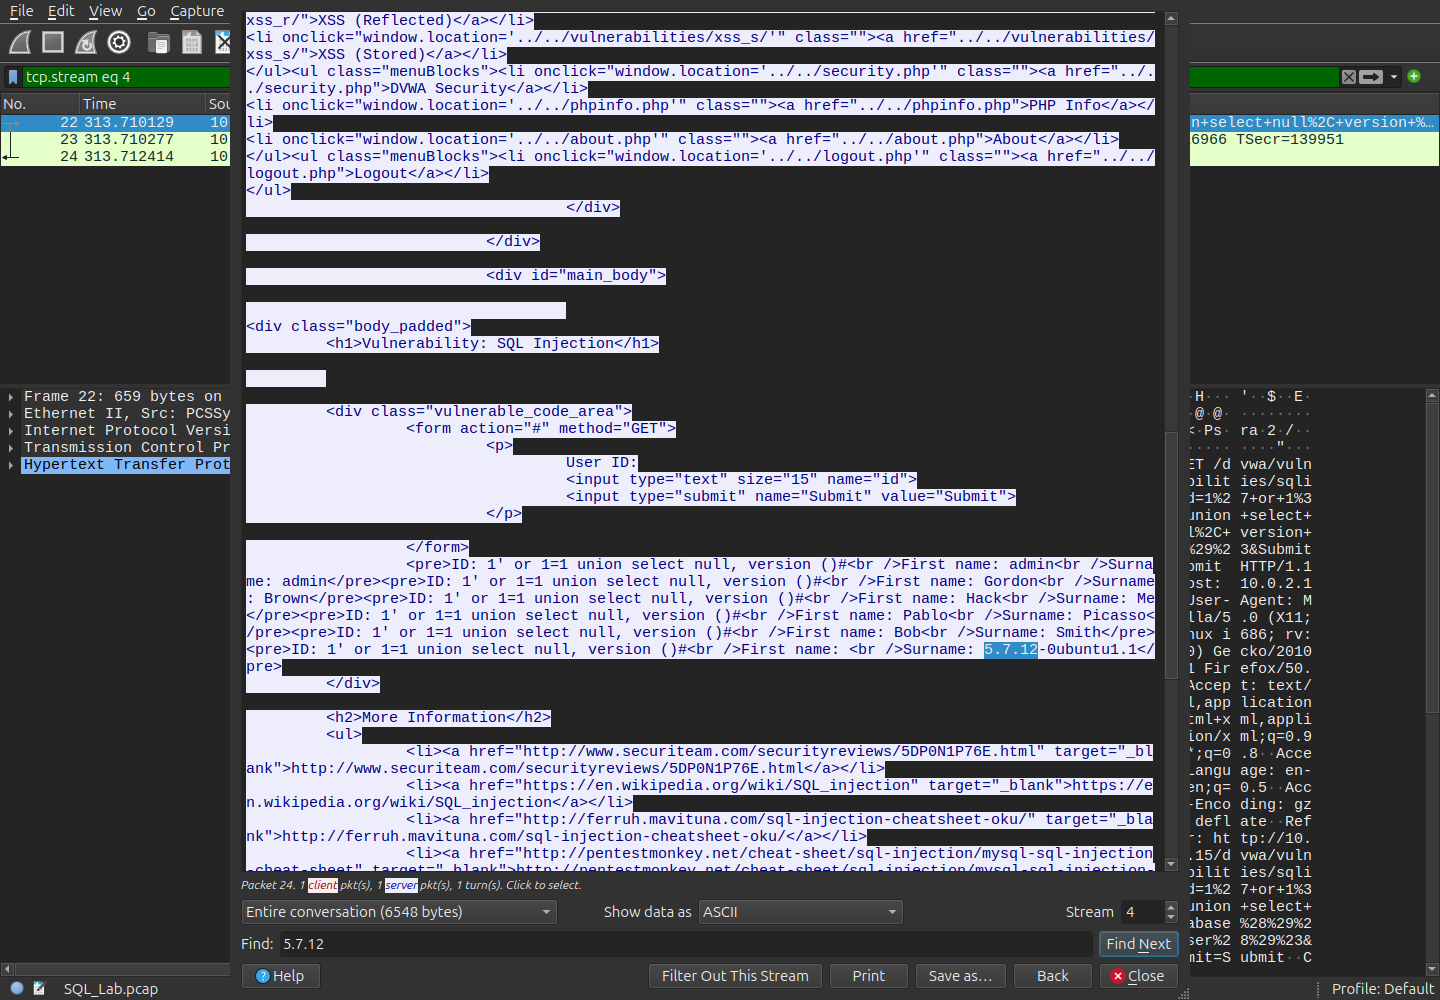
\includegraphics[width=\textwidth]{04_version.png}
\caption{Identificador de versión de MySQL obtenido mediante version().}
\end{figure}

\subsection{Paso 5: tablas y columnas}
El paquete 25 solicita:
\begin{verbatim}
1' or 1=1 union select null, table_name
from information_schema.tables#
\end{verbatim}
La respuesta del paquete 27 enumera tablas visibles para la cuenta de conexión,
entre ellas \texttt{users}. La amplitud de la salida se debe a consultar
\texttt{information\_schema.tables} sin restringir el esquema; \texttt{NULL}
solo completa una de las dos columnas requeridas por \texttt{UNION}.

\textbf{¿Qué haría la consulta modificada de la consigna?}
\begin{verbatim}
1' OR 1=1 UNION SELECT null, column_name
FROM INFORMATION_SCHEMA.columns WHERE table_name='users'
\end{verbatim}
Enumeraría los \textbf{nombres de las columnas} de las tablas llamadas
\texttt{users} que resulten visibles, agregándolos al resultado de la consulta
original. Permitiría conocer la estructura para preparar consultas posteriores;
no obtiene directamente el contenido de esas columnas. Al no filtrar por
\texttt{table\_schema}, puede incluir tablas homónimas de varias bases. Además,
el fragmento debe cerrar o comentar correctamente el resto de la sentencia
original para funcionar: la versión propuesta omite el comentario final.
Esta modificación es una pregunta conceptual y no aparece ejecutada en el PCAP.

\begin{figure}[H]
\centering
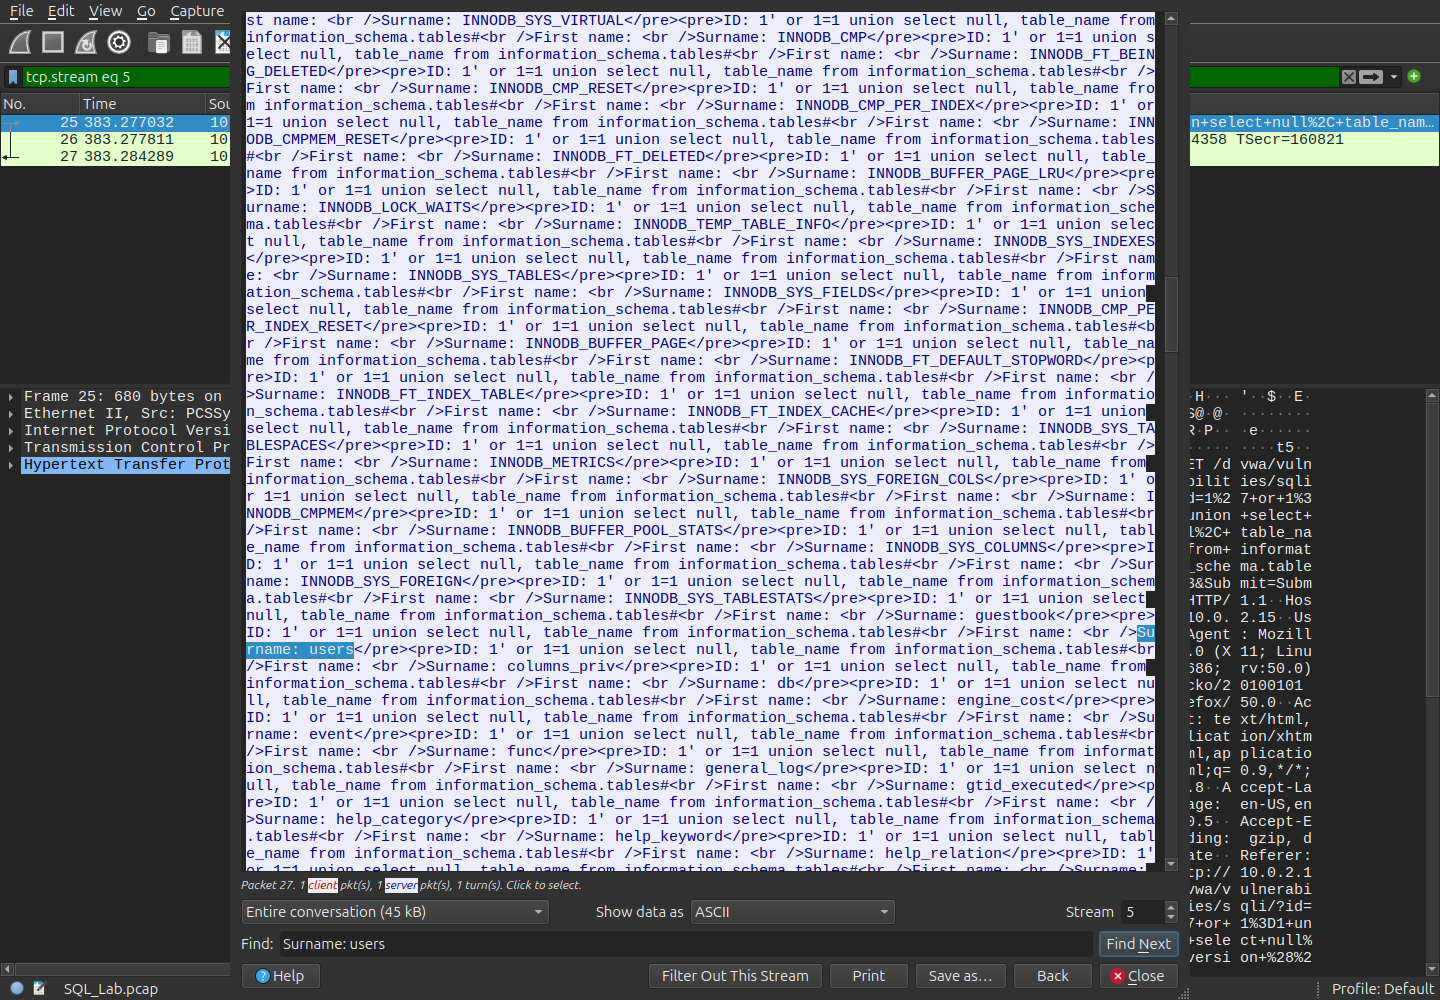
\includegraphics[width=\textwidth]{05_tablas.png}
\caption{Enumeración de tablas: se localiza users en la respuesta HTTP.}
\end{figure}

\subsection{Paso 6: usuarios y hashes de contraseñas}
La solicitud del paquete 28 contiene:
\begin{verbatim}
1' or 1=1 union select user, password from users#
\end{verbatim}
La respuesta del paquete 30 asocia el usuario \textbf{1337} con el siguiente hash:
\begin{center}
\texttt{8d3533d75ae2c3966d7e0d4fcc69216b}
\end{center}
La contraseña en texto plano
compatible con ese hash es \textbf{charley}. Se verificó localmente:
\begin{center}
\texttt{MD5(charley) = 8d3533d75ae2c3966d7e0d4fcc69216b}
\end{center}
El cálculo utiliza los bytes UTF-8 de la palabra, sin salto de línea.
El script \path{evidencias/verificar_hash.py} reproduce esta comprobación.
Una función hash no se descifra: se prueban candidatos o se buscan coincidencias
en tablas precalculadas. CrackStation describe este último mecanismo para hashes
sin sal~\cite{crackstation}.

Se ingresó el hash en el formulario de CrackStation. El sitio devolvió una
coincidencia exacta, identificó el tipo como \texttt{md5} y mostró
\texttt{charley} en la columna de resultado. La captura documenta esa consulta
y la comprobación local aporta una verificación independiente.

\begin{figure}[H]
\centering
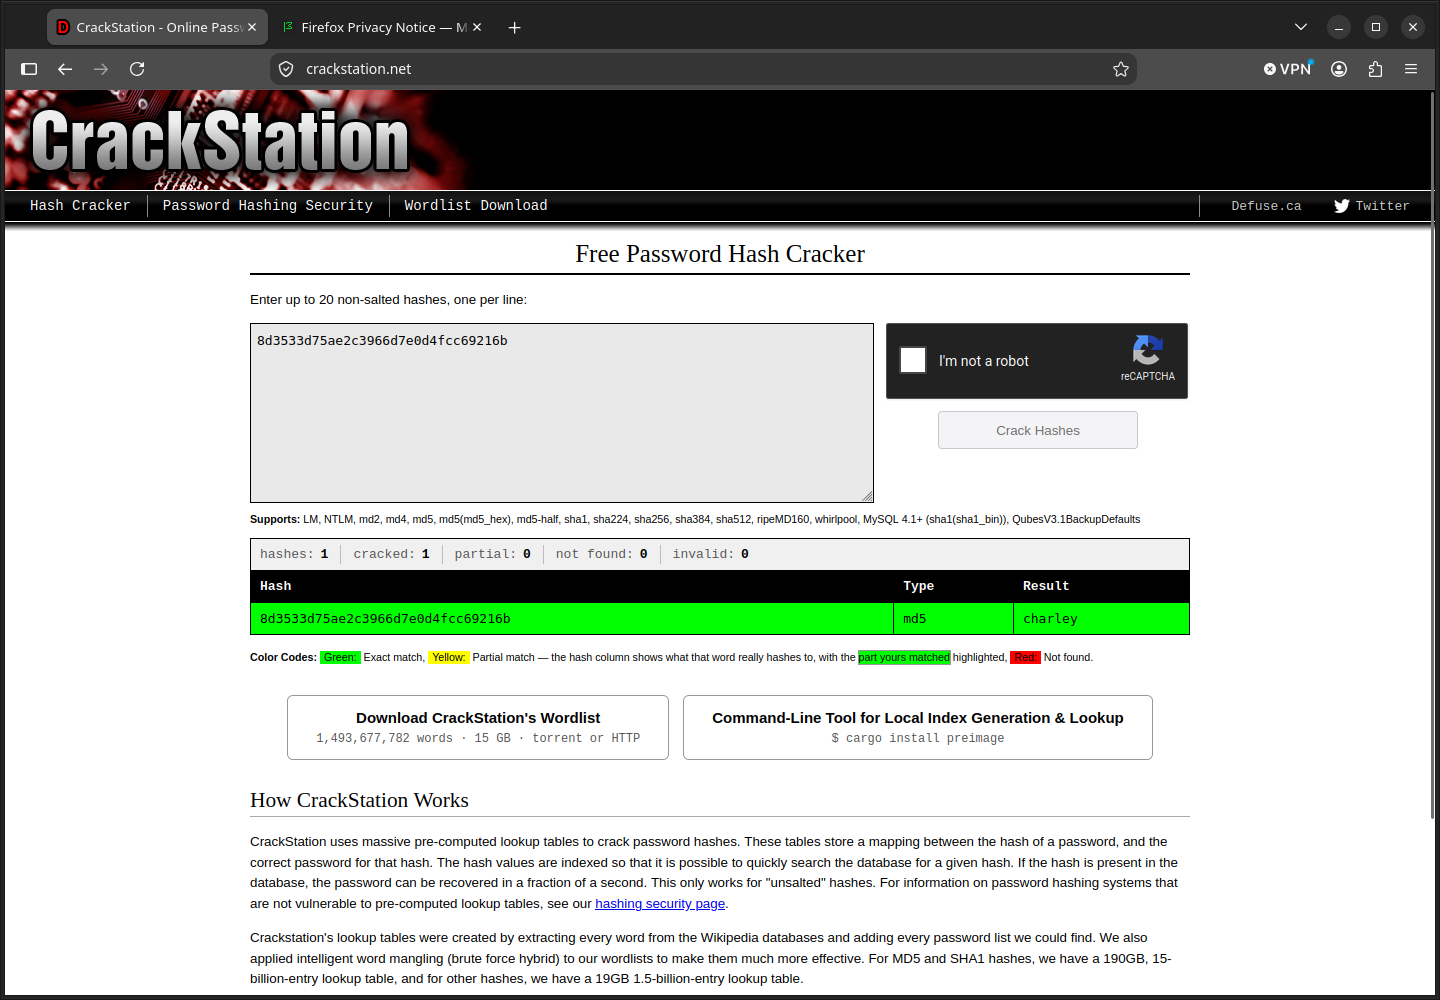
\includegraphics[width=\textwidth]{08_crackstation.png}
\caption{Resultado real de CrackStation: coincidencia exacta del hash MD5 con charley.}
\end{figure}

\begin{figure}[H]
\centering
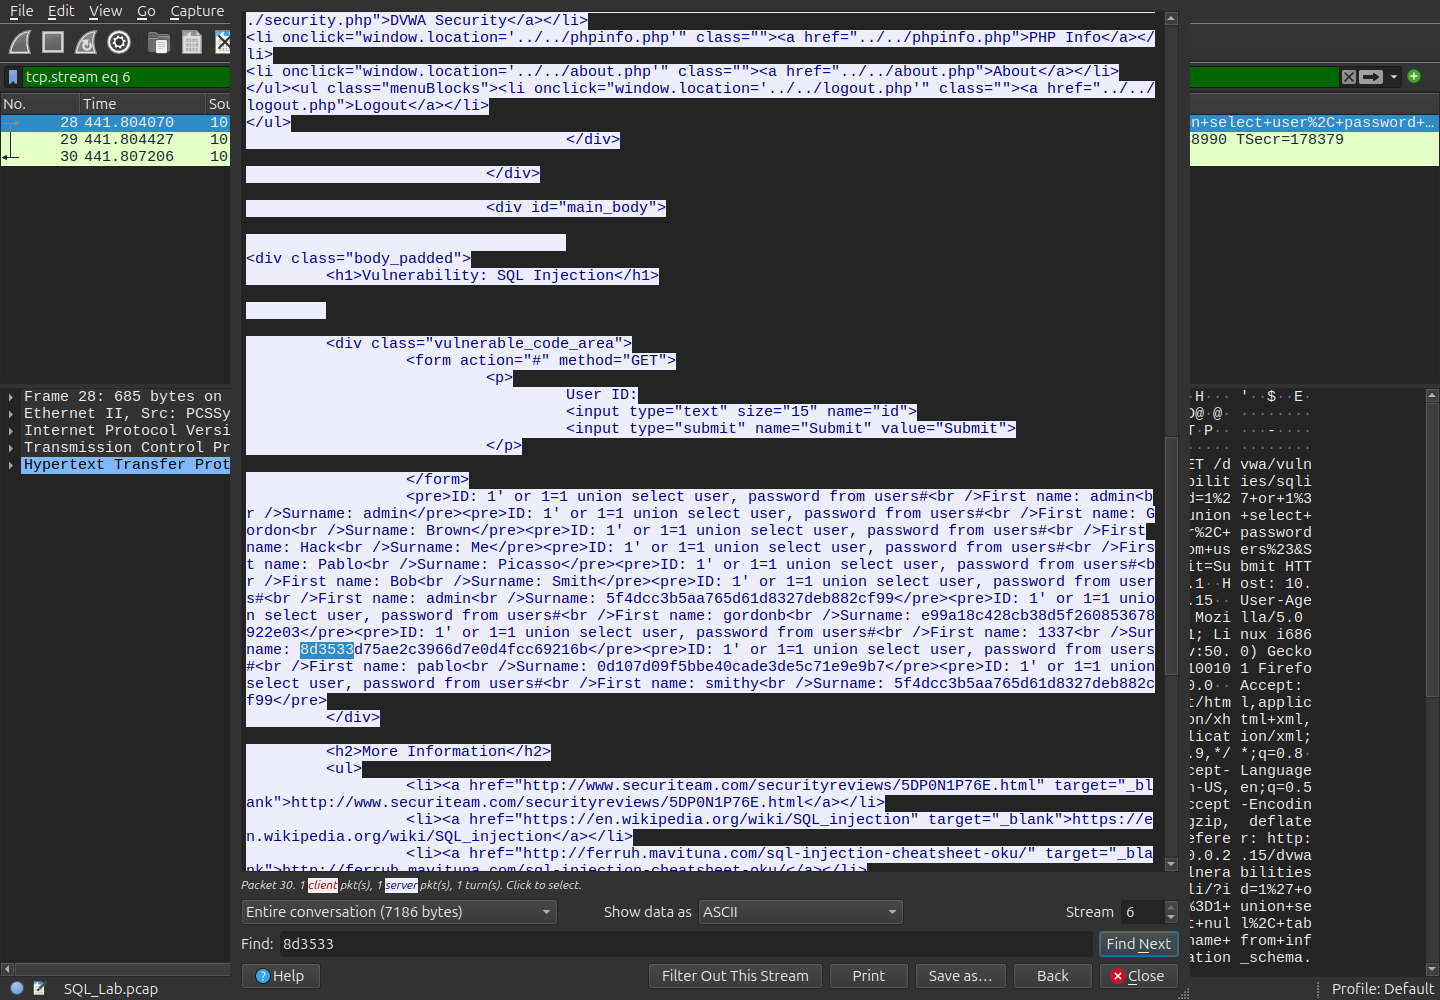
\includegraphics[width=\textwidth]{06_hash.png}
\caption{Extracción de usuarios y hashes: el usuario 1337 aparece asociado al hash solicitado.}
\end{figure}

\begin{figure}[H]
\centering
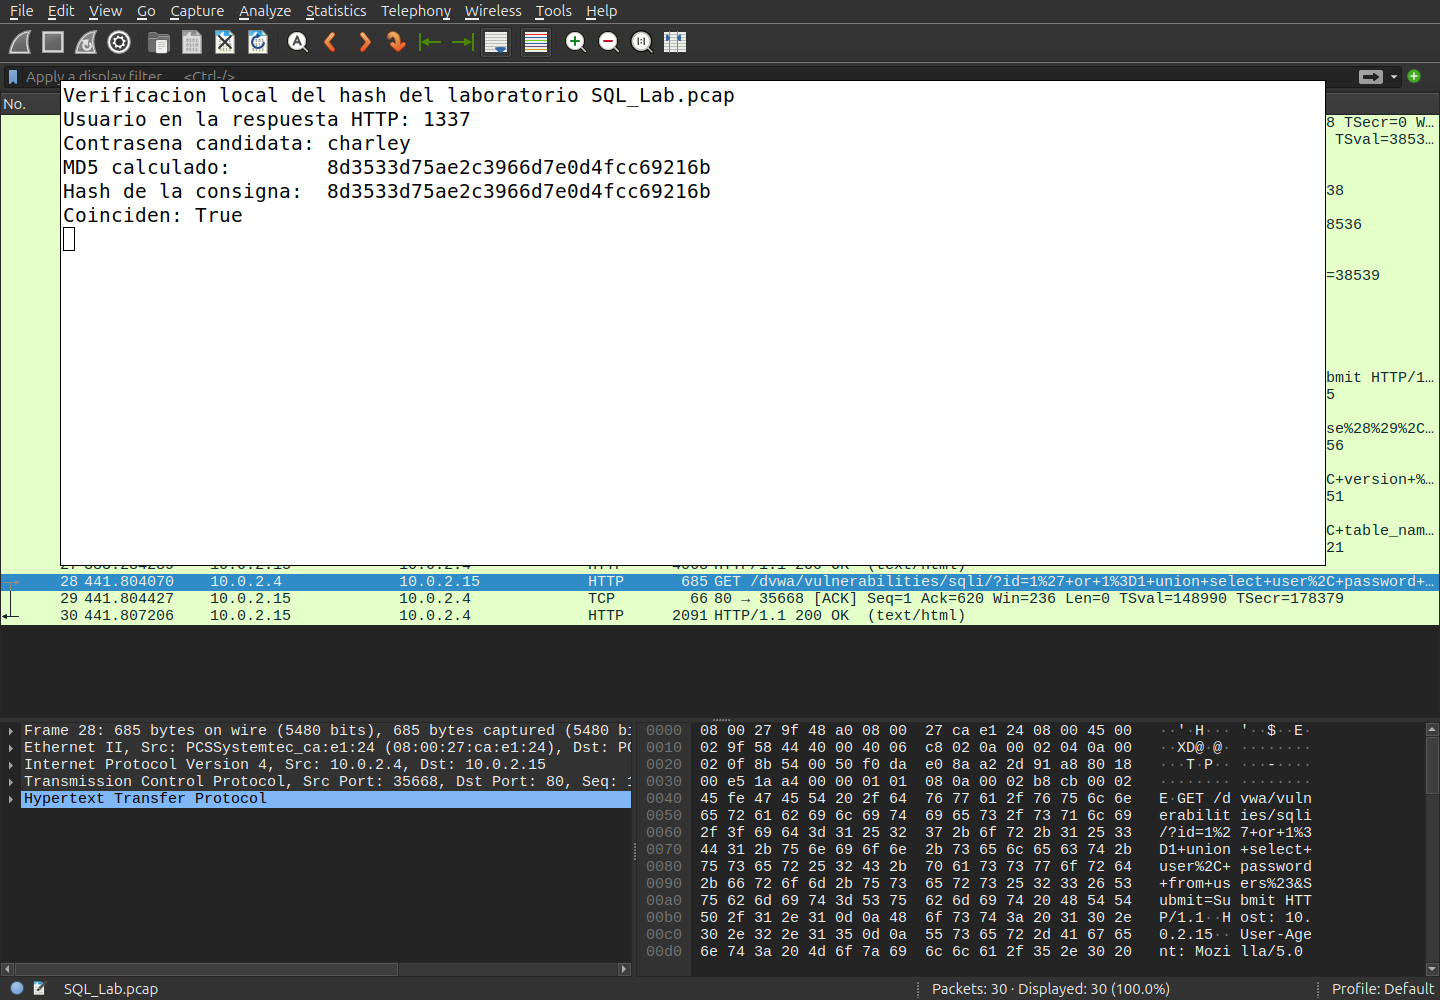
\includegraphics[width=\textwidth]{07_verificacion_local.png}
\caption{Ejecución real de la verificación local de MD5 para la contraseña charley.}
\end{figure}

\section{Entregable}
\subsection{¿Cuál es el riesgo de que las plataformas utilicen SQL?}
El uso de SQL no constituye por sí mismo una vulnerabilidad. El riesgo aparece
cuando la aplicación incorpora entradas del usuario al texto de una consulta
sin separar los datos de las instrucciones. Un atacante puede cambiar su
significado y acceder a información fuera del alcance previsto~\cite{owasp}.

En este caso se observa pérdida de confidencialidad: exposición de metadatos,
usuarios y hashes. En otras aplicaciones, según la consulta vulnerable y los
permisos de la cuenta, una inyección también podría permitir alterar o borrar
datos, eludir controles de acceso o afectar la disponibilidad. El PCAP analizado
no demuestra borrado, modificación de registros ni ejecución de malware.
El valor \texttt{root@localhost} observado justifica revisar los privilegios de
la aplicación, aunque el nombre de cuenta por sí solo no enumera sus permisos.

\subsection{Métodos para evitar ataques de inyección SQL}
A partir de la guía de OWASP~\cite{owasp}, se proponen estas medidas:
\begin{enumerate}[noitemsep]
\item \textbf{Consultas preparadas con parámetros.} Mantener fija la estructura
SQL y pasar los valores por separado, sin concatenar la entrada del usuario.
\item \textbf{Validación mediante listas de valores permitidos.} Exigir el tipo
y rango esperados para User ID. Los identificadores dinámicos, como nombres de
tablas, deben elegirse entre opciones controladas por el programa.
\item \textbf{Mínimo privilegio.} Usar una cuenta exclusiva con acceso solo a las
tablas y operaciones necesarias. Esto reduce el daño posible de una falla.
\item \textbf{Procedimientos almacenados seguros.} Parametrizar las entradas
también dentro de ellos y evitar construir SQL dinámico por concatenación.
\end{enumerate}
La validación complementa la parametrización. Escapar caracteres manualmente
no debe ser la defensa principal.

\section{Conclusiones}
El análisis reconstruyó la progresión desde una prueba de entrada hasta la
extracción de hashes. Se identificaron las IP, la base dvwa, la cuenta de
conexión root@localhost, la versión de MySQL y la asociación entre 1337 y el
hash de charley. Las capturas y los flujos extraídos respaldan estos resultados.
La prevención debe centrarse en separar datos e instrucciones mediante
parámetros, validar entradas y restringir los privilegios de la aplicación.
CrackStation confirmó la contraseña y el cálculo local de MD5 reprodujo
exactamente el hash extraído.

\begin{thebibliography}{9}
\bibitem{consigna}
Material de la actividad, \emph{Práctica de laboratorio: Ataque a una base de
datos mySQL}. Consigna y archivo \texttt{SQL\_Lab.pcap} suministrados.
\bibitem{owasp}
OWASP, \emph{SQL Injection Prevention Cheat Sheet}.
\url{https://cheatsheetseries.owasp.org/cheatsheets/SQL_Injection_Prevention_Cheat_Sheet.html}.
Consulta: 23 de septiembre de 2026.
\bibitem{crackstation}
CrackStation, \emph{Free Password Hash Cracker}, sección How CrackStation Works.
\url{https://crackstation.net/}. Consulta de la página informativa:
23 de septiembre de 2026.
\end{thebibliography}
\end{document}
